%% This is file `elsarticle-template-1-num.tex',
%%
%% Copyright 2009 Elsevier Ltd
%%
%% This file is part of the 'Elsarticle Bundle'.
%% ---------------------------------------------
%%
%% It may be distributed under the conditions of the LaTeX Project Public
%% License, either version 1.2 of this license or (at your option) any
%% later version.  The latest version of this license is in
%%    http://www.latex-project.org/lppl.txt
%% and version 1.2 or later is part of all distributions of LaTeX
%% version 1999/12/01 or later.
%%
%% Template article for Elsevier's document class `elsarticle'
%% with numbered style bibliographic references
%%
%% $Id: elsarticle-template-1-num.tex 149 2009-10-08 05:01:15Z rishi $
%% $URL: http://lenova.river-valley.com/svn/elsbst/trunk/elsarticle-template-1-num.tex $
%%
\documentclass[titlepage,11pt]{article}
%\documentclass[longtitle,preprint,12pt]{elsarticle}

%% Use the option review to obtain double line spacing
%%\documentclass[preprint,review,12pt]{elsarticle}

%% Use the options 1p,twocolumn; 3p; 3p,twocolumn; 5p; or 5p,twocolumn
%% for a journal layout:
%%\documentclass[final,1p,times,]{elsarticle}
%% \documentclass[final,1p,times,twocolumn]{elsarticle}
%% \documentclass[final,3p,times]{elsarticle}
%% \documentclass[final,3p,times,twocolumn]{elsarticle}
%% \documentclass[final,5p,times]{elsarticle}
%% \documentclass[final,5p,times,twocolumn]{elsarticle}

%% The graphicx package provides the includegraphics command.
\usepackage{graphicx}
%% The amssymb package provides various useful mathematical symbols
\usepackage{amssymb,amsmath,amsthm}
\usepackage{bbold}
%\usepackage[latin1]{inputenc}
%% The amsthm package provides extended theorem environments
%% \usepackage{amsthm}
\usepackage{braket}
\usepackage{lineno}
\usepackage{authblk}
\usepackage{color}
\usepackage{geometry}
\usepackage{subfigure}
\usepackage{tikz}
\usepackage{adjustbox}
\usepackage{tkz-euclide}
\usepackage{pst-solides3d}
\usetikzlibrary{matrix}
\usepackage{tikz-3dplot}
\usepackage{wrapfig}
%encoding
%--------------------------------------
\usepackage[utf8]{inputenc}
\usepackage[T1]{fontenc}
%--------------------------------------
 
%Portuguese-specific commands
%--------------------------------------
%\usepackage[portuguese]{babel}
%------------------------------
\geometry{left=3cm,right=2cm,top=2.5cm,bottom=2.5cm}
\renewcommand{\thefootnote}{\alph{footnote}}	
\DeclareMathOperator{\Ima}{Im}
\usepackage{amsthm}

\theoremstyle{plain}% default
\newtheorem{thm}{Theorem}[section]
\newtheorem{lem}[thm]{Lemma}
\newtheorem{prop}[thm]{Proposition}
\theoremstyle{definition}
\newtheorem{defn}[thm]{Definition}
\newtheorem{exmp}[thm]{Example}
\theoremstyle{remark}
\newtheorem{rem}[thm]{Remark}



\begin{document}

%% Title, authors and addresses

\title{Relat\'{o}rio de Atividades / Activities Report\\\textsc{Beyond Topological Order in Arbitrary Dimensional Quantum Systems - Geometrical States}}


	\author[a]{Juan Pablo Ibieta-Jimenez}
  \author[a]{ Paulo Teotonio-Sobrinho (Advisor)}
\affil[a]{Departamento de F\'{\i}sica Matem\'{a}tica, Instituto de F\'{\i}sica, Universidade de S\~{a}o Paulo, S\~{a}o Paulo SP, Brasil}
\maketitle

\begin{abstract}
We present the annual report concerning academic and research activities for the II-2017 and I-2018 academic terms in the Ph.D. program of the DFMA-IFUSP at the \emph{Universidade de S\~{a}o Paulo}. Moreover, we emphasize the progress in the research project and outline the activity plan for the following academic year.
\end{abstract}

%\begin{keyword}
%Topological Order \sep Lattice Gauge Theory \sep Exactly solvable models
%% keywords here, in the form: keyword \sep keyword

%% MSC codes here, in the form: \MSC code \sep code
%% or \MSC[2008] code \sep code (2000 is the default)

%\end{keyword}

%\end{frontmatter}

%%
%% Start line numbering here if you want
%%
%\linenumbers

%% main text
\section{A Synopsis of the Research Project}\label{S:1}

The discovery of the \textbf{Fractional Quantum Hall Effect} (FQH) \cite{Laughlin} revealed the existence of intricate phases of matter whose internal orders or ``patterns'' do not have any relation with any kind of symmetries (or the breaking of them) and thus cannot be described by the usual Ginzburg-Landau symmetry-breaking scheme. They are said to be \textbf{Topologically ordered} because, in general, their ground state is degenerate and this degeneracy depends on the topology of the space \cite{Haldane,Wen3,Wen4} that can not be modified by perturbations or impurities \cite{Wen1}. Thus, only a change in the internal pattern or topological order  can induce a change in the ground state degeneracy. The special features of topologically ordered systems extend to their excitations as they exhibit characteristic properties such as the fractionalization of the charge and anyonic statistics \cite{Oshikawa-Senthil, Oshikawa}. 

In the past few years there has been a major interest on the study of these phases of matter via a detailed analysis of exactly solvable lattice models that exhibit the features of having \textbf{topological order}. The simplest example is the so called \textbf{Toric Code} model introduced by A. Kitaev in \cite{Kitaev2} which is constructed as a many body interacting system defined over a 2-dimensional lattice. It exhibits the features of a topologically ordered system as its ground state is 4-fold degenerate when the lattice is embedded on the surface of a Torus, hence part of its name. The degeneracy is protected from local perturbations that come as the elementary excitations of the model. These elementary excited states can be interpreted as quasi-particle anyonic excitations located at the vertices and faces of the lattice, they display both bosonic and fermionic statistics when braided among themselves. This model can be interpreted as a particular lattice gauge theory \cite{Kogut} where the gauge group is the abelian $\mathbb{Z}_2$  group \cite{Kitaev2}. Furthermore, for any finite group $G$, in \cite{Kitaev2} Kitaev introduces a more general class of models called \textbf{Quantum Double Model} (QDM)  defined through a Hamiltonian that is written as a sum of mutually commuting projectors \cite{Drinfeld,majid2000,dijkgraaf,Propitius}. The elementary excitations of this models are anyons whose fusion and braiding properties depend on the specific choice of the group $G$ giving rise to the possibility of having non-abelian anyons that can be used to implement a fault-tolerant quantum computation process \cite{kauffman,collins,preskill,pachos}, where unitary transformations are obtained by the braiding of anyons and the final measurement is performed by the joining of pairs of excitations. 

The problem of classifying topological phases of matter is of fundamental importance the condensed matter and the quantum information communities. Topological phases are effectively described by Topological Quantum Field Theories (TQFTs) \cite{Witten,Atiyah88}. Thus, in principle, an identification of TQFTs that can possibly describe gapped phases of gauge theories can be used as a means of classification of topological phases. In the absence of any further global symmetry and for the case of gapped phases of finite $1$-gauge theories, an incomplete list of TQFTs has been given by Dijkgraaf and Witten \cite{Witten,Dijkgraaf90}. Concretely, Dijkgraaf-Witten topological actions with gauge group $G$ have been used to distinguish gapped phases of matter with global symmetry group $G$. These are known as symmetry protected topological (SPT) phases \cite{Wen-Gu09,Chen12,Oshikawa10,Oshikawa12,Fidkowsky11,LevinGu} and are described by the group cohomology classification of SPT phases \cite{Chen-Wen13}. A more general classification of SPT phases was proposed in \cite{Kapustin14}. 


On the other hand, it is clear that there are theories that go beyond the Dijkgraaf-Witten scheme and could involve both higher gauge fields and higher gauge symmetries. Recently, higher dimensional generalizations of TQFTs have attracted interest from both, within the context of topological phases of matter and within the context of quantum error correction codes.  In \cite{Kapustin13} a class of TQFTs involving $1$-form and $2$-form gauge fields has been studied using $2$-groups instead of the usual notion of  $1$-groups. Consequently, the existence of gapped phases of matter that are protected by a $2$-group instead of a $1$-group symmetry is proposed. Moreover, along these lines, in \cite{Bullivant16}, a Hamiltonian formulation of the Yetter’s homotopy $2$-type TQFT \cite{Yetter} was constructed with the aim of understanding $(3+1)$ topological phases of matter. Also, it is worth to mention the works of \cite{Yoshida16}, where bosonic lattice realizations of SPT phases with higher form symmetry are presented, and \cite{Yoshida15,Yoshida17}, where is discussed their connection to fault-tolerant logical gates in topological quantum codes. 


In \cite{higher} we construct and study a class of models that could live in arbitrary dimensions and go beyond $1$-gauge theories and, therefore, escape from previous classification schemes. These theories involve higher gauge fields and symmetries in all possible dimensions. The notion of a gauge group is replaced by a more general mathematical object, namely, a chain complex of abelian groups. As a consequence, the notion of \textit{gauge configuration} is replaced by the notion of \textit{maps between two chain complexes}. In this mathematical framework is quite natural to construct a Hamiltonian formulation of higher lattice gauge theories that can be defined in arbitrary dimensions. The class of Hamiltonian models obtained from this picture are shown to have a degenerate ground state subspace whose basis elements are in one-to-one correspondence with the cohomology classes having coefficients in the chain complex of abelian groups \cite{Brown}. Furthermore, this formalism allows to explicitly show that the ground state degeneracy (GSD) is a topological invariant, for which we give a closed formula in terms of the order of the $0$-th cohomology group with coefficients in the chain complex of abelian groups. Moreover, due to a theorem by Brown \cite{Brown}, the GSD can be understood as exhibiting contributions from each dimension, therefore exhibiting the different intrinsic \textit{topological orders} involved.  


The models describe gapped phases of abelian gauge theories and can be interpreted as describing topological phases of matter \cite{Wen04,Sarma08,Anderson87} when taking the geometrical chain complex to be a discretization of a compact manifold. Thus, our construction allows us to get a variety of models exhibiting intrinsic topological order \cite{Wen89,Wen90,LevinWen} that can be thought of as prototypical models of topological phases of matter in higher dimensions. Great interest on such kind of models arose due to possible applications in fault tolerant quantum computation \cite{Kitaev2,Nayak08,Freedman03}. In particular, these models can be used to store quantum information as quantum error correction codes. In fact, a particular case of the latter is studied in \cite{Hastings}, where the chain complex of abelian groups is chosen to have only one non trivial component. This case results in a family of quantum CSS stabilizer codes \cite{CalderbankCSS} (We refer to \cite{Devitt} for a brief review on quantum codes and related topics). Quantum stabilizer codes use the ground state subspace to encode quantum information, thus the number of logical qubits is related to the GSD of the particular model. It was already noted in the literature that such codes can be written in terms of Homology \cite{Bombin07,Bombin13,Bravyi14}. Since the models presented in this piece of work are written in the language of Homology, they are naturally interpreted as the higher dimensional versions of the so called homological quantum error correction codes \cite{Bravyi98,Vrana15,Anderson13hom}. Furthermore, the closed formula we have obtained for the GSD of the model determines both the coding space and the labels of the logical operators.


% The contents of this paper are organized as follows. In Section \ref{sec:Math} we establish the mathematical apparatus that will be used to construct the models, namely, we define $\text{hom}(C,G)$ a cochain complex and its dual, where $C$ and $G$ are two chain complexes of Abelian groups. The cohomology groups $H^n (C,G)$ are defined, where the $0$-th cohomology is of utter importance due to a theorem by Brown \cite{Brown}, that decomposes the former into simpler cohomologies in each dimension of the chain. In Section \ref{sec:Model}, we define the actual models. Concretely, the Hilbert space $\mathcal{H}$ and its states are defined. The local operators and all their important algebraic relations are proven and by the end of the Section, the Hamiltonian operator $H:\mathcal{H}\rightarrow\mathcal{H}$ is defined. In Section \ref{sec:GSD} we study the ground state subspace $\mathcal{H}_0 \in \mathcal{H}$ as a suitable way to prove our main result, which is that there is a one-to-one relation between the basis elements of the ground state subspace $\mathcal{H}_0$ and the elements of the $0$-th cohomology group of the cochain complex $hom(C,G)$. The analysis is presented in three parts: first, we show the measurement operators of the ground states; secondly, we show the relation of these operators and the elements of the dual of $H^0 (C,G)$; and thirdly, we briefly discuss a suitable isomorphism that identifies these elements as the quantum parameters of the quantum model presented. The final Section \ref{sec:Disc} is a discussion of the work presented and links to other topics. There are also three appendices intended to supply additional information to make the present work as self contained as possible. % In appendix A we give a brief review of Simplicial Homology. In appendix B we define the notion of Dual Groups from the representation theory of abelian groups. Finally, in appendix C we show two expansions corresponding to the local operators of the theory that are used in the proof of the final result.



\subsection{Objective}\label{Ss:1}
The formalism developed in \cite{pramod} allows for the obtention of a large class of models where the bosonic degrees of freedom at vertices are coupled with gauge fields at links. Many such models can be got by the mere choice of the main ingredients, i.e., the gauge group $G$ and a $\mathbb{C}[G]$-module $(V_n, \mu)$. Aiming at a higher gauge theory interpretation, such models can be understood as a $0,1$-gauge theory. Since degrees of freedom are associated to both $0-cells$ (vertices) and $1-cells$ (links). In \cite{kazuothesis,ricardo} a very similar formalism is constructed for (3+1) topological phases using a $2$-group as the gauge group. This is, a $1,2$-gauge theory for topological phases of matter was constructed. In this case, degrees of freedom are associated to the $1-cells$ (links) and $2-cells$ (plaquettes). Taking these ideas into consideration, in \cite{higher} we constructed a Hamiltonian model for topological phases of matter in arbitrary dimensions. Furthermore, the notion of gauge group is promoted to a more general mathematical structure, that of a \textit{chain complex of abelian groups}. In this new framework, it can be shown \cite{higher} that the ground state degeneracy is a topological invariant of an abstract co-chain complex. In this sense, the ground state of such models is completely characterized and understood from the $0$-th cohomology group associated to such co-chain complex. Moreover, a theorem due to Brown \cite{Brown} relates this rather abstract cohomology group with the usual cohomology groups, enabling for a natural geometrical interpretation of the ground state subspace. 

Recently, we have found that by considering some of these fields as having only \emph{classical configurations}, the otherwise purely topological models now become sensitive to the geometry of the manifold upon which they are defined. This is showcased, as in the purely topological case, in the ground states of the Hamiltonian models, as we will show in the next section for a particular example. This fact has turned our attention to these new class of models that, we believe, are related to some other new findings in the topological phases of matter community. In particular, there is a strong interest in a new class of quantum states called \emph{fracton} phases \cite{chamon05,bravyi11,castelnovo12,haah11,bravyi13,yoshida13,vijay15,vijay16,vijay17,shirley17,rahul18}. Some characteristic of fracton phases include elementary excitations with restricted mobility and in some cases a ground state degeneracy that explicitly depends on the geometry of the manifold \cite{slagle17}. The latter has caught our attention as the higher gauge theories constructed in \cite{higher} can be modified to obtain a source of models with a geometrical dependence of the ground state degeneracy. The systematic construction of such models consists on restricting some $l$-constituents of the $n$-gauge configurations to be classical; This leads to equivalence classes of Hamiltonian models, some of which, have a geometrical dependence of the ground state degeneracy.  The construction of the models starting from the full higher gauge theories, the analysis of the unitary classes of Hamiltonians and the study of the geometrical models constitute the main contents of the Ph.D. research project. In this sense, the main objective of the research project is to characterize the topological and geometrical phases coming from the procedure of partially freezing the degrees of freedom. This endeavor is partially achieved since the construction of the models and their characterization with respect to the appearance of geometrical phases or not is known, as we will show in the next section. There are, however, some details that have to be concealed before considering the project as finished, they include:
\begin{itemize}
\item A Proof that the geometrical states are indeed the ground states of such Hamiltonians.
\item A brief study of the excited states, paying special attention to the mobility restrictions that appear in fracton phases.
\item To fit the description of the models into the formalism developed in \cite{higher}.
\end{itemize}


\section{Progress and Preliminary Results}
We divide this section in two parts. In the first half we intend to give a brief review of the class of models constructed in \cite{higher}. The formalism developed in \cite{higher} is extremely powerful to treat lattice gauge theories in arbitrary dimensions and with arbitrary assignment of abelian gauge groups to the $n$-cells of the lattice. It includes a plethora of models already known in the literature in a compact but rather abstract way. We describe the models through several examples, since we find this is the best way to understand the spirit of both the theory and the construction; In addition, we will use these models to show, in detail , how the procedure of making some degrees of freedom classical provides a new class of models. Among them there are Hamiltonians whose ground states are sensitive to the geometry of the manifold the model is embedded in a particular way. Thus, in the second part we include the preliminary results concerning the construction and the properties of the geometrical models, we do this through an example.


\subsection{Abelian Higher Gauge Theories}
The models constructed in \cite{higher} consist on the Abelian versions of Higher Gauge Theories on the lattice, in the Hamiltonian formalism. Very similar to the way the Quantum Double Models (QDMs) with  group $G$ are understood as the Hamiltonian formulation of a (2+1) lattice gauge theory with gauge group $G$ \cite{Bais,Dijkgraaf90}. In this sense, the QDMs are a natural starting point.
\subsubsection{1-Gauge Theory (2D): QDMs}\label{sec:QDMs}
 The standard construction of the model \cite{Kitaev2} defines a many body interaction Hamiltonian over a two dimensional oriented lattice $\Lambda_\Sigma$ (usually squared) that can come from the discretization of a 2-manifold $\Sigma$.  Moreover, a local Hilbert space $\mathcal{H}_l=\mathbb{C}(G)$ is associated to each edge $l\in \Lambda^{(1)}$, where $\mathbb{C}(G)$ is the group algebra of the finite group $G$ i.e., the vector space over the complex numbers spanned by the basis elements $\{\Ket{g}\}_{g \in G}$ labeled by group elements $g \in G$. The dimension of this local vector space is $\dim \mathcal{H}_l=|G|$, the order of the group. Consequently, the full Hilbert space, with the usual inner product,  is naturally constructed as being the tensor product of all local spaces $\mathcal{H}_i$, namely,
\begin{equation}\label{eq:HilbertQDM}
 \mathcal{H}:=\bigotimes_{i \in \Lambda} \mathcal{H}_i.
\end{equation}
An arbitrary basis state of this space is written $\ket{g_1,g_2, \dots, g_N}$, with $g_i \in G$, this is, basis elements of $\mathcal{H}$ are \emph{classical gauge configurations}.
The Hamiltonian of the model is a sum of two types of local projection operators that commute with each other, commonly referred to as \emph{vertex} and \emph{plaquette} operators:
\begin{equation}
H_{QDM}=-\sum_{v \in \Lambda^{(0)}} A_v - \sum
_{p \in \Lambda^{(2)}} B_p,
\end{equation}
where $A_v$ and $B_p$ are the vertex and plaquette operators, respectively. These operators implement the local gauge symmetry and the local flatness condition, respectively and are defined by:
\begin{align}
 A_v := \frac{1}{|G|}\sum_{g \in G}A_v^g, &\ \label{eq:Av1G} \  \text{where: } \\
 A_v^g \quad \vcenter{\hbox{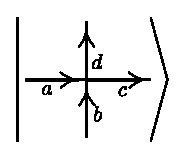
\includegraphics[scale=0.65]{AvQDMket1.eps}}}\ &= \ \vcenter{\hbox{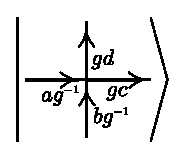
\includegraphics[scale=0.65]{AvQDMket2.eps}}}, \nonumber \\
 B_p \quad \vcenter{\hbox{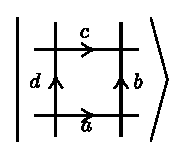
\includegraphics[scale=0.65]{BpQDMket1.eps}}}\ &= \delta(abc^{-1}d^{-1},e)\ \vcenter{\hbox{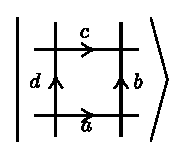
\includegraphics[scale=0.65]{BpQDMket1.eps}}},
\end{align}
with $e\in G$ is the identity element. One of the topological features of the QDMs is encoded in the invariant subspace $\mathcal{H}_0:= \{ \ket{\psi} \in \mathcal{H}\ | \ A_v\ket{\psi} = \ket{\psi}\ \text{and }\ B_p\ket{\psi}=\ket{\psi}, \ \forall v,p \in \Lambda\}$, in particular, its dimension coined ``Ground State Degeneracy" $GSD=|\mathcal{H}_0|$ is of topological nature as it counts the homotopy classes of the manifold $\Sigma$. This is well showcased in the most known QDM, the Toric Code (TC) \cite{kitaev2}, where the gauge group is the cyclic group $\mathbb{Z}_2$.

Up to this point, we already exhibited what we consider the three more important ingredients in a lattice gauge theory, namely, the classical gauge configurations that span $\mathcal{H}$, the local gauge transformations, implemented by $A_v$, in charge of quantum entanglement, and the $B_p$ operator that implements the local flatness condition by measuring the holonomy along an elementary plaquette and checking if is equal to the identity element, $e \in G$. We make emphasis on these three conceptsas they are the ones to be generalized in order to construct what we call an Abelian Higher Gauge Theory. More precisely, a gauge configuration can be thought of as a map that assigns a group element to each edge $l \in \Lambda^{(1)}$, an elementary gauge transformation is labeled by a group element in $G$ and is localized at (the co-boundary of) a vertex.

\subsubsection{2-Gauge Theory (2D)}\label{sec:2gauge}
We are ready to make a first generalization of the models described in \S \ref{sec:QDMs}. In this particular case, we consider the possibility of having dynamical degrees of freedom living at the plaquettes as well as the usual degrees of freedom that live on links of the lattice. In the present construction the geometric input data of the model will come from a simplicial chain complex $(C,\partial)$. Nevertheless, more general mathematical structures can be considered, such as graphs, $\Delta$-complexes  or CW-complexes \cite{Hatcher}. We choose simplicial complexes for no other reason than simplicity. Thus, let $X$ be a compact 2-manifold and $K=K(X)$ the simplicial complex associated to such manifold; Specifically, $K_0$ is the set of 0-simplices (vertices), $K_1$ is the set of 1-simplices (links) and $K_2$ the set of 2-simplices (faces). Consequently, $C_n$ stands for the Abelian group of $n$-chains, i.e., the Abelian group generated by $K_n$.
More precisely, we are considering the following chain complex:
 \begin{equation}\label{eq:GeomChainCompAbQDM}
0 \xrightarrow{\partial_{3}} C_{2} \xrightarrow{\partial_2}  C_{1}  \xrightarrow{\partial_1} C_0 \xrightarrow{\partial_0} 0,
 \end{equation}
where $0$ stands for the trivial group and the $\partial_i, \ \i=1,2$ are the usual boundary operators of the simplicial chain complex. 
The sets of $n$-simplices $K_n$ are taken to be finite and in this case they are non-empty for $n=0,1,2$ only. This is important in order to have a finite dimensional Hilbert space as we will see in the following lines. The Hilbert space $\mathcal{H}$ construction is very similar to the QDMs, as the basis states that span   
$\mathcal{H}$ are labeled by \emph{gauge configurations}. To extend the notion of gauge configuration for the model at hand, we consider two Abelian groups $G_1$ and $G_2$. The first one labels the local basis states at edges $\mathcal{H}_l, \
l \in K_1$, whose basis states are $\{\ket{g}\}, \ g \in G_1$. Likewise, the group $G_2$ labels the local basis at plaquettes $\mathcal{H}_p, \ p \in K_2$, with basis states $\{\ket{\alpha}\}, \alpha \in G_2$. Naturally, the total Hilbert space is given by:
\begin{equation}\label{eq:Hilb2G}
\mathcal{H}:=\bigotimes_{l\in K_1} \mathcal{H}_l \bigotimes_{p \in K_2} \mathcal{H}_p
\end{equation}
The coupling between both kinds of degree of freedom is achieved through a group homomorphism $\partial:G_2 \rightarrow G_1$. Notice that, in this case, an arbitrary gauge configuration is labeled by both Abelian groups $G_1$ and $G_2$. This means that a gauge configuration can be thought of as a map $f=\{f_1,f_2\}$ as shown in Fig. \ref{fig:2gch}
\begin{figure}[!h]
 %			\begin{adjustbox}{max size={0.95 \textwidth}{0.95 \textheight}}
            \centering
 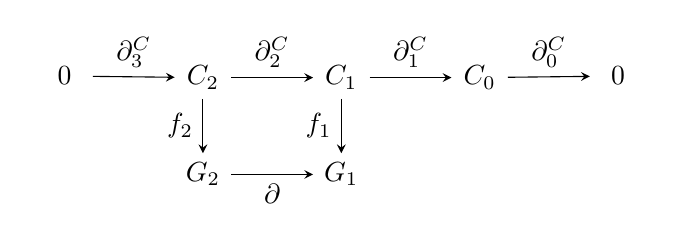
\begin{tikzpicture}
  \matrix (m) [matrix of math nodes,row sep=2em,column sep=3em,minimum width=2em]
  { 0 & C_{2} & C_{1} & C_{0} & 0 \\
      & G_2 & G_1 &   \\};
  \path[-stealth]
    (m-1-1) edge node [above] {$ \partial^C_3 $} (m-1-2)
    (m-1-2)	edge node [above] {$ \partial^C_2 $} (m-1-3)
            edge node [left] {$ f_2 $} (m-2-2)
    (m-1-3) edge node [above] {$ \partial^C_1 $} (m-1-4)
    		edge node [left] {$f_{1}$} (m-2-3)
    (m-1-4) edge node [above] {$ \partial^C_0 $} (m-1-5)
    		%edge node [left] {$ f_0 $} (m-2-4)
    %(m-2-1) edge node [below] {$ \partial^G_3 $} (m-2-2)
    (m-2-2) edge node [below] {$ \partial $} (m-2-3);
    %(m-2-3) edge node [below] {$ \partial^G_1 $} (m-2-4);
%    (m-2-4) edge node [below] {$ \partial^G_0 $} (m-2-5);
\end{tikzpicture}
%\end{adjustbox}
\caption{\label{TCcomplex} A gauge configuration thought of as a set of maps $f=\{f_1,f_2\}$}\label{fig:2gch}
\end{figure}


Let \(x_i \in K_1, \ i=1, \dots, |K_1|\) and \(y_j \in K_2, \ j=1, \dots, |K_2|\), an arbitrary basis state of \(\ket{f} \in \mathcal{H}\) is written $\ket{f}=\ket{f_1(x_1),\dots, f_1(x_{|K_1|}),f_2(y_1),\dots f_2(y_{|K_2|})}$, where \(f_1(x_i) \in G_1\) and \(f_2(y_j) \in G_2\).

The Hamiltonian of the model is very similar to \(H_{QDM}\) since it consists on a sum of local commuting projectors and they perform gauge transformations and 1-holonomy measurements. In particular, 
\begin{equation}\label{eq:H2G}
H_{2G}=-\sum_{v \in K_0} A_v -\sum_{l \in K_1} A_l - \sum
_{p \in K_2} B_p,
\end{equation}
the first kind of operators, $A_v$, get labeled by the vertices of the simplicial complex, $v \in K_0$, their definition is given through its action on basis states and it is exactly the same as the in QDMs (cf \S \ref{sec:QDMs}), 
\begin{align}
 A_v := \frac{1}{|G_1|}\sum_{g \in G_1}A_v^g, &\ \label{eq:Av2G}  \text{where: } \\
 A_v^g \quad \vcenter{\hbox{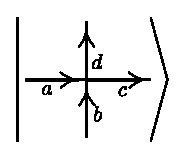
\includegraphics[scale=0.65]{AvQDMket1.eps}}}\ &= \ \vcenter{\hbox{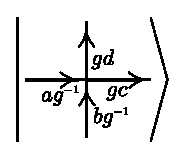
\includegraphics[scale=0.65]{AvQDMket2.eps}}}, \nonumber
\end{align}
where $g \in G_1$. There is a second kind of gauge transformation, $A_l$, which we call \emph{2-gauge transformation}, it is labeled by links of the simplicial complex $l \in K_1$ and defined by:
\begin{align}
 A_l := \frac{1}{|G_2|}\sum_{\beta \in G_1}A_l^{\beta}, &\ \label{eq:Al2G} \text{where: } \\
 A_l^\beta \quad \vcenter{\hbox{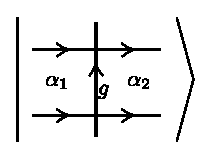
\includegraphics[scale=0.65]{Al2Gket1.eps}}}\ &= \ \vcenter{\hbox{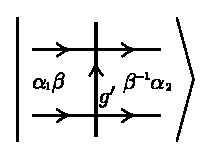
\includegraphics[scale=0.65]{Al2Gket2.eps}}}, \nonumber
\end{align}
where $\beta \in G_2$ and $g^{\prime}= \partial (\beta) g$. This is, the 2-gauge transformation acts on the actual link and the two faces adjacent to the link. Finally, the last kind of operators are similar to the plaquette operators in the QDMs, however, they have a slight modification that comes from the generalized notion of 1-holonomy of the theory, given by:
\begin{align}\label{eq:Bp2G}
 B_p \quad \vcenter{\hbox{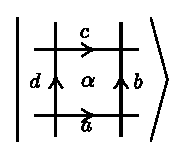
\includegraphics[scale=0.65]{Bp2Gket1.eps}}}\ &= \delta(abc^{-1}d^{-1},\partial(\alpha))\ \vcenter{\hbox{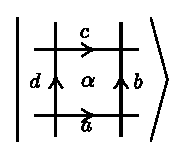
\includegraphics[scale=0.65]{Bp2Gket1.eps}}},
\end{align}
where $a,b,c,d \in G_1$ and $\alpha \in G_2$. It can be shown that the above operators form a set of mutually commuting projectors. The topological properties of the ground state subspace $\mathcal{H}_0 \subset \mathcal{H}$ is encoded in the ground state projector, which in this case has the form:
\begin{align}
P_0:=\prod_{v}A_v\prod_{l}A_l\prod_{p}B_p,
\end{align}
that projects the basis of $\mathcal{H}$ into the basis of $\mathcal{H_0}$. In particular, the ground state degeneracy of the model is given by the trace of this projector, $\text{GSD}=\text{tr}(P_0)$.
\begin{exmp}

Consider a model defined on the surface of $S_2$ where the degrees of freedom are labeled by $G_1=\mathbb{Z}_2=\{1,-1\}$ and $G_2=\mathbb{Z}_4=\{1,i,-1,-i\}$. More precisely, the local Hilbert spaces of 1-gauge degrees of freedom, are located at 1-simplices (links) $l \in K_1$ and labeled by elements of $\mathbb{Z_2}$, i.e., $\mathcal{H}_l=\mathbb{C}(\mathbb{Z}_2)$. Whereas, the local Hilbert space of the 2-gauge degrees are located at the 2-simplices $p \in K_2$, this is, $\mathcal{H}_p=\mathbb{C}(\mathbb{Z}_4)$. We still need to define a group homomorphism $\partial:G_2 \rightarrow G_1$, which in this case we take to be defined by $\partial(i)=-1$.  The local operators can be written in terms of the usual Pauli matrices for the $\mathbb{Z}_2$ degrees of freedom and the shift and clock operators for $\mathbb{Z}_4$.

The Hamiltonian is the one in Eq.(\ref{eq:H2G}) and it is not hard to realize that the ground state subspace is spanned by the following two states:
\begin{align*}
\ket{GS_1} &=\prod_{v}A_v\prod_{l}A_l\bigotimes_{l \in K_1}\ket{1}_l \bigotimes_{p \in K_2} \ket{1}_p,\\
\ket{GS_{-1}} &=\prod_{v}A_v\prod_{l}A_l\bigotimes_{l \in K_1}\ket{1}_l \bigotimes_{p \neq p^{\prime}} \ket{1}_p \otimes \ket{-1}_{p^{\prime}},
\end{align*}
where the  $\ket{1}_l \in \mathcal{H}_l$ and $1 \in \mathbb{Z}_2$; Similarly, $\ket{1}_p \in \mathcal{H}_p$ and $1 \in \mathbb{Z}_4$. Note that the two states only differ from each other by a configuration of a single (arbitrary) plaquette, $p^{\prime}$. This is because no local 2-gauge transformation can map between the two states. 
 The two ground states are identified from each other by measuring the global 2-holonomy. In this case, the operator that performs such measurement is given by:
\[h_2:=\prod_{p}Z_p, \quad \forall \ p\in \mathcal{L},\]
where $Z_p$ is the $\mathbb{Z}_4$ clock operator acting at plaquette $p$, clearly,
\begin{align*}
h_2\ket{GS_1}=&\ket{GS_1},\\
h_2\ket{GS_{-1}}=&-\ket{GS_{-1}},
\end{align*}
Notice that the ground states can be stabilized (protected) by the bulk when the model is defined on $S^2\times I$, where $I$ is the interval, since in this case no local perturbation can lift the degeneracy.
\end{exmp}


\subsubsection{3-Gauge Theory (3D)} To illustrate how the notions of gauge configurations, gauge transformations and holonomy measurements are generalized in the higher gauge theory scheme, we consider a \emph{3-gauge theory} in 3 dimensions. Going one dimension up provides us the possibility of including degrees of freedom on the volumes (3-simplices) of the following simplicial complex:
\begin{equation}\label{eq:GeomChainCompAbQDM}
0 \xrightarrow{\partial_{4}} C_3 \xrightarrow{\partial_{3}} C_{2} \xrightarrow{\partial_2}  C_{1}  \xrightarrow{\partial_1} C_0 \xrightarrow{\partial_0} 0,
 \end{equation}
where $C_3$ is the Abelian group of 3-chains (formal sums of 3-simplices in $K_3$).  Therefore, we are placing degrees of freedom at links $l \in K_1$, plaquettes $p \in K_2$ and "cubes" $c \in K_3$. Consequently, we need three Abelian groups $G_1$, $G_2$ and $G_3$ to label the local basis. This makes the total Hilbert space to be of the following form:
\begin{equation}\label{eq:Hilb3G}
\mathcal{H}:=\bigotimes_{l\in K_1} \mathcal{H}_l \bigotimes_{p \in K_2} \mathcal{H}_p \bigotimes_{c \in K_3} \mathcal{H}_c,
\end{equation}
where $\mathcal{H}_l:= \mathbb{C}(G_1)$ are the local Hilbert spaces at links $l \in K_1$,  $\mathcal{H}_p:= \mathbb{C}(G_2)$ at plaquettes and $\mathcal{H}_c:= \mathbb{C}(G_3)$ at cubes. Moreover, we also need group homomorphisms that couple the degrees of freedom, in other words, we consider the following abstract chain complex of Abelian groups:
\begin{equation}\label{eq:Abcc3G}
 0\xrightarrow{\partial_4}  G_3\xrightarrow{\partial_3}G_2\xrightarrow{\partial_2} G_1\xrightarrow{\partial_1} 0,
\end{equation}
where $0$ stand for the trivial group. With this setup, a gauge configuration is just a collection of maps $f=\{f_i\}_{i=1,2,3}$ as shown in Fig.\ref{fig:3Gconf}.

\begin{figure}[h]
\centering
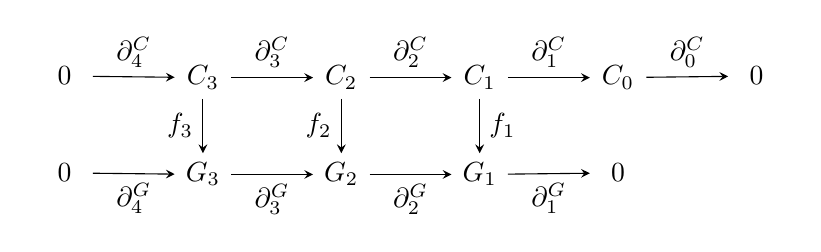
\begin{tikzpicture}
  \matrix (m) [matrix of math nodes,row sep=2em,column sep=3em,minimum width=2em]
  {   0 & C_{3} & C_{2} & C_{1} & C_{0} & 0  \\
      0 & G_3 & G_{2} & G_{1} & 0  \\};
  \path[-stealth]
    (m-1-1) edge node [above] {$\partial^C_{4}$} (m-1-2) 
    (m-1-2) edge node [above] {$\partial^C_{3}$} (m-1-3)
            edge node [left] {$f_3$} (m-2-2)
    (m-1-3) edge node [above] {$\partial^C_{2}$} (m-1-4)
    		edge node [left] {$f_{2}$} (m-2-3)
    (m-1-4) edge node [above] {$\partial^C_{1}$} (m-1-5)
    (m-1-5) edge node [above] {$\partial^C_{0}$} (m-1-6)
    %(m-1-5) edge node [right] {$f_0$} (m-2-5)
    (m-1-4) edge node [right] {$f_{1}$} (m-2-4)
    (m-2-1) edge node [below] {$\partial^G_{4}$} (m-2-2)
    (m-2-2) edge node [below] {$\partial^G_{3}$} (m-2-3)
    (m-2-3) edge node [below] {$\partial^G_{2} $} (m-2-4)
    (m-2-4) edge node [below] {$\partial^G_{1}$} (m-2-5);
    %(m-2-5) edge node [below] {$\partial^G_{0}$} (m-2-6);
\end{tikzpicture}
\caption{\label{fig:3Gconf} A classical gauge configuration of the 3-gauge theory seen as a collection of maps $\{f_i\}$.}
\end{figure}
The Hamiltonian of the model is similar to the ones in the previous sections, in the sense that it consists of operators that either perform gauge transformations or measure different kinds of holonomies. In particular, the inclusion of degrees of freedom at volumes (3-simplices) results in a new term in the Hamiltonian that measures the 2-holonomy around cubes as well as a term that enhances 3-gauge transformations, as we will see. The Hamiltonian is given by:

\begin{equation}\label{eq:H3G}
H= -\sum_{v}A_v -\sum_{l}A_l -\sum_{p}A_p -\sum_{p}B_p -\sum_{c}B_c,
\end{equation}
Where $A_v$, $A_l$, and $A_p$ are the operators in charge of performing 1,2 and 3-gauge transformations, respectively. Whereas $B_p$ and $B_c$ measure 1- and 2-holonomies, respectively. The 1-gauge transformation operator $A_v$ is labeled by vertices $v \in K_0$ and has the following form:
\begin{equation}\label{eq:3GAv}
A_v=\dfrac{1}{|G_1|}\sum_{g \in G_1} A_v^{g},
\end{equation}
where $A_v^g$ acts as in Eq.(\ref{eq:Av2G}), this is, on the links adjacent to vertex $v$; This operator establishes the local 1-gauge symmetry of the theory and acts on 1-gauge degrees of freedom only. 

\begin{figure}[h!]
\centering
\subfigure[$A_l$ operator.]{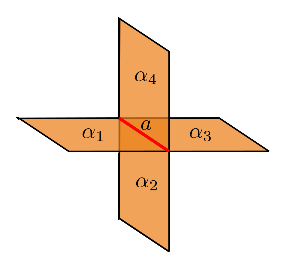
\includegraphics[scale=0.65]{Al3Gacts2.eps}}\hspace{30pt}
\subfigure[$A_p$ operator.]{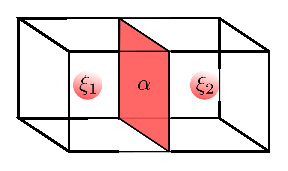
\includegraphics[scale=0.65]{Ap3Gacts.eps}}

%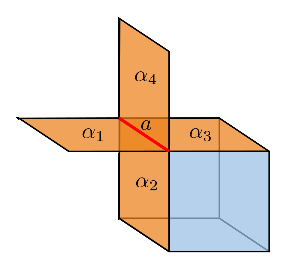
\includegraphics[scale=0.6]{Al3Gacts.eps}
\caption{The support of $A_l$ and $A_p$ on the lattice is shown, respectively, for arbitrary link $l \in K_1$ and plaquette $p \in K_2$.}
\label{fig:Al3G}
\end{figure}

Let us go now to the operator that implements the \emph{2-gauge transformation}, $A_l$, similar to the one of Eq.(\ref{eq:Al2G}) as it gets labeled by links $l \in K_1$ and given by:
\begin{equation}\label{eq:Al3G}
A_l=\dfrac{1}{|G_2|}\sum_{\beta \in G_2} A_l^{\beta},
\end{equation}
let us write $\ket{ a, \alpha_1,\alpha_2,\alpha_3,\alpha_4, \dots}$ for an arbitrary basis state in $\mathcal{H}$, whose configuration corresponds to that of Fig.\ref{fig:Al3G}; The action of $A_l^\beta$ on this state is given by:
\begin{align*}
A_l^{\beta}\ket{a, \alpha_1,\alpha_2,\alpha_3, \alpha_4, \dots} &= \\ & \hspace{-55pt} = \ket{\partial_{2}(\beta)a, \alpha_1\beta^{-1},\alpha_2\beta^{-1},\beta\alpha_3,\beta\alpha_4, \dots}
\end{align*}
Similarly, the operator $A_p$ implements the \emph{3-gauge} transformations, it gets labeled by 2-simplices (plaquettes), $p \in K_2$, of the simplicial complex. Given by:
\begin{equation}
A_p=\dfrac{1}{|G_3|}\sum_{\zeta \in G_3}A_p^{\zeta},
\end{equation} 
where the elementary 3-gauge transformation, $A_p^{\zeta}$, labeled by a group element $\zeta \in G_3$, is defined by its action on arbitrary basis states:
\begin{align*}
A_p^{\zeta}\ket{\alpha, \xi_1, \xi_2, \dots}= \ket{\partial_3(\zeta)\alpha, \xi_1\zeta, \zeta^{-1}\xi_2, \dots},
\end{align*}
the configuration of the state $\ket{ \alpha, \xi_1, \xi_2, \dots} \in \mathcal{H}$ is depicted in Fig. \ref{fig:Al3G}(b).
The above operators implement all types of gauge transformations in the theory, the next kind of operators in Eq.(\ref{eq:H3G}) are in charge of measuring the generalized notion of holonomies of the 3-gauge theory. Just as in the 2-gauge theory, the 1-holonomy is measured by the plaquette operator $B_p$, defined in Eq.(\ref{eq:Bp2G}). A 3-gauge theory also has another kind of holonomy, which we call 2-holonomy; It is measured on a 3-simplex (cube) by going along the surface and collecting the 2-gauge degrees of freedom sitting on plaquettes and the 3-gauge degree of freedom at the cube itself, this is schematized in Fig.(\ref{fig:Bc3G}). 
The $B_c$ operator measures this quantity and checks if it is equal to identity $1 \in G_2$ as follows:
\begin{align}
B_c\ket{\alpha_1,\alpha_2,\alpha_3,\alpha_4,\alpha_5,\alpha_6, \xi, \dots}=  
 \delta(\prod_{i=1}^{6} \alpha_i,\partial(\xi))\ket{\alpha_1,\alpha_2,\alpha_3,\alpha_4,\alpha_5,\alpha_6, \xi,\dots },
\end{align}
where $\alpha_i \in G_2,\ i=1,\dots, 6$ are the 2-gauge fields living on the faces of the cube and $\xi \in G_3$ the 3-gauge field living at the cube itself.
\begin{figure}[h!]
\centering
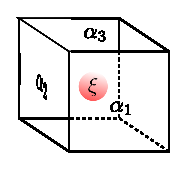
\includegraphics[scale=0.8]{Bc3Gacts.eps}
\caption{The 2-holonomy is measured by collecting the 2-gauge degrees of freedom lying along the surface of the cube together with the 3-gauge field that lives in the cube itself.}\label{fig:Bc3G}
\end{figure}


\begin{exmp}
We consider a 3-gauge theory defined on a discretization of $S^3$. Let us place $\mathbb{Z}_4$ degrees of freedom at volumes, faces and links of the lattice. This is, we have the following abstract chain complex of groups $G_1=G_2=G_3=\mathbb{Z}_4$,
\begin{equation}\label{eq:3dcc}
 1\xrightarrow{\partial_4}  G_3\xrightarrow{\partial_3}G_2\xrightarrow{\partial_2} G_1\xrightarrow{\partial_1} 1,
\end{equation}
where $\partial_1$ and $\partial_4$ are trivial and $\partial_2$, $\partial_3$ are both defined by
$$\partial_j(i)=-1, \ \ j=2,3,$$
where $i$ is the generator of $\mathbb{Z}_4=\{1,i,-1,-i\}$.
The Hamiltonian of the model is the one in Eq.(\ref{eq:H3G}),
%%%%%%%%%%%%%%%%%%%%%% For split version
%The Hamiltonian is written as a sum of mutually commuting projectors, namely,

\begin{equation*}
H= -\sum_{v}A_v -\sum_{l}A_l -\sum_{p}A_p -\sum_{p}B_p -\sum_{c}D_c,
\end{equation*}
Where $A_v$, $A_l$, and $A_p$ are the operators that perform 1,2 and 3-gauge transformations, respectively. Whereas $B_p$ and $B_c$ measure the 1- and 2-holonomies, respectively. 
%The  1-gauge transformation is the usual one and can be written is terms of the shift operator $X$ of $\mathbb{Z}_4$:
%%%%%%%%% Non-abelian version
%The Hamiltonian of the model is written as a sum of mutually commuting projectors, namely,
%\begin{equation}
%H= -\sum_{v}A_v-\sum_{p}B_p -\sum_{c}D_c,
%\end{equation}
%as in the previous cases, the above operators perform gauge transformations and measure fake 1 and 2 fake holonomies. In particular,  the $A_v$ operator performs 1-gauge transformations and it is defined as:
%\begin{equation}
%A_v:=A_v^{\text{1-g}}\prod_{l\in\text{star}(v)}A_l^{\text{2-g}}\prod_{f\in\text{star}(v)}A_f^{\text{3-g}},
%\end{equation}
%again, $A_v^{\text{1-g}}$ is the 1-gauge transformation and for this particular model it is given by:

%\begin{multline*}
%A_v=\dfrac{1}{6}(\mathbb{1}_{l_1}\otimes\mathbb{1}_{l_2}\otimes\mathbb{1}_{l_3}
%\otimes\mathbb{1}_{l_4}\otimes\mathbb{1}_{l_5}
%\otimes\mathbb{1}_{l_6}+ \\ + X_{l_1}\otimes X_{l_2}\otimes X_{l_3}\otimes X^3_{l_4}\otimes X^3_{l_5}\otimes X^3_{l_6} + \\
%+ X^2_{l_1}\otimes X^2_{l_2}\otimes X^2_{l_3}\otimes X^2_{l_4}\otimes  X^2_{l_5}\otimes X^2_{l_6} + \\ + X^3_{l_1}\otimes X^3_{l_2}\otimes X^3_{l_3}\otimes X_{l_4}\otimes X_{l_5}\otimes X_{l_6}),
%\end{multline*}
%where $\{l_i\}_{i=1}^6$ are labels for the 6 links that meet at vertex $v$.
%The 2-gauge transformations are performed by the $A_l$ operators labeled by the links of the lattice since their non trivial support consists on the link $l$ and the four faces that meet at $l$ (Fig.(\ref{fig:Al3G})) in the following way:
%\begin{multline*}
%A_l=\dfrac{1}{4}(\mathbb{1}_{l}\otimes\mathbb{1}_{p_1}\otimes\mathbb{1}_{p_2}
%\otimes\mathbb{1}_{p_3}\otimes\mathbb{1}_{p_4}+X^2_{l}\otimes X_{p_1}\otimes X_{p_2} \otimes X^3_{p_3} \otimes X^3_{p_4}+ \\
%+\mathbb{1}_l \otimes X^2_{p_1} \otimes X^2_{p_2} \otimes X^2_{p_3}\otimes X^2_{p_4}  +X^2_{l}\otimes X^3_{p_1} \otimes X^3_{p_2} \otimes X_{p_3} \otimes X_{p_4})
%\end{multline*}
%Finally, the 3-gauge transformations are performed by the $A_p$ operators, they are labeled by the plaquettes of the lattice as their non trivial action support consists on a face $p$ and the two volume degrees of freedom adjacent to $p$ (see Fig.(\ref{fig:Al3G})), i.e., for this particular example the operator is given by:
%\begin{equation*}
%A_p=\dfrac{1}{4}(\mathbb{1}_p \otimes \mathbb{1}_{c_1}\otimes \mathbb{1}_{c_2}+ 
%X_{c_1}\otimes X^2_{p}\otimes X^3_{c_2} + X^2_{c_1}\otimes \mathbb{1}_{p}\otimes %X^2_{c_2}+ X^3_{c_1}\otimes X^2_{p}\otimes X_{c_2}),
%\end{equation*}
%where  $X$ is the shift matriz of $\mathbb{Z}_4$:


%As in the previous examples, the plaquette operator $B_p$ projects to the trivial fake 1-holonomy subspace and it is given by:
%\begin{multline*}
%B_p=\dfrac{1}{4}(\mathbb{1}_p \otimes \mathbb{1}_{l_1} \otimes \mathbb{1}_{l_2} \otimes \mathbb{1}_{l_3} \otimes \mathbb{1}_{l_4} + Z^2_{p}\otimes Z_{l_1}\otimes Z_{l_2} \otimes Z^3_{l_3} \otimes Z^3_{l_4} + \\ + \mathbb{1}_p \otimes Z^2_{l_1} \otimes Z^2_{l_2} \otimes Z^2_{l_3} \otimes Z^2_{l_4} +  Z^2_{p}\otimes Z^3_{l_1}\otimes Z^3_{l_2} \otimes Z_{l_3} \otimes Z_{l_4}),
%\end{multline*}
%on the other hand, the \textit{cube operator} $D_c$ projects to the trivial fake 2-holonomy:
%\begin{multline*}
%B_c=\frac{1}{4}(\mathbb{1}_c \otimes\mathbb{1}_{f_1} \otimes\mathbb{1}_{f_2} \otimes\mathbb{1}_{f_3} \otimes\mathbb{1}_{f_4} \otimes\mathbb{1}_{f_5} \otimes\mathbb{1}_{f_6}+ Z^2_{c}\otimes Z_{f_1} \otimes Z_{f_2} \otimes Z_{f_3}\otimes Z^3_{f_4} \otimes Z^3_{f_5} \otimes Z^3_{f_6}+ \\ + \mathbb{1}_c \otimes Z^2_{f_1} \otimes Z^2_{f_2} \otimes Z^2_{f_3} \otimes Z^2_{f_4} \otimes Z^2_{f_5} \otimes Z^2_{f_6}+ Z^2_{c} \otimes Z^3_{f_1} \otimes Z^3_{f_2} \otimes Z^3_{f_3} \otimes Z_{f_4} \otimes Z_{f_5} \otimes Z_{f_6}),
%\end{multline*}
%the $X$ and $Z$ matrices in all the above operators are the $\mathbb{Z}_4$  shift and clock matrices. 

The model has two ground states when defined in a discretization of the 3-sphere $S^3$. They are obtained by applying 1,2,3 gauge transformations on non-equivalent seed states, i.e.,
\begin{align*}
\ket{G_1}=&\prod_{v}A_v\prod_{l}A_l\prod_{p}A_p\bigotimes_{l}\ket{1}_l\bigotimes_{p}\ket{1}_p\bigotimes_{c}\ket{1}_c, \\
\ket{G_2}=&\prod_{v}A_v\prod_{l}A_l\prod_{p}A_p\bigotimes_{l}\ket{1}_l\bigotimes_{p}\ket{1}_p\bigotimes_{c\neq c^\prime}\ket{1}_c\otimes\ket{-1}_{c^\prime},
\end{align*}
the second seed state corresponds to having a volume degree of freedom $\ket{-1}$ on an arbitrary cube $c^{\prime}$. Clearly the seed states are not gauge equivalent since there is no 3-gauge transformation that can map between the two seed states. In this case the ground states are distinguished from each other by the global 3-holonomy operator defined as:
\begin{equation}\label{eq:glob3h}
h_3:=\prod_{c} Z_c,
\end{equation}
it can be checked by a straightforward computation that:
\begin{align*}
h_3\ket{G_1}=&\ket{G_1}, \\
h_3\ket{G_2}=&-\ket{G_2}.
\end{align*}
%The ground state degeneracy of the model coincides with our homology counting scheme, namely, the third homology group of the abstract chain complex of eq.(\ref{eq:3dcc}) is given by:
%$$H_3=\dfrac{\text{ker} \partial_3}{\text(Im) \partial_4}=\dfrac{\mathbb{Z}_2}{\{\ \}}\simeq \mathbb{Z}_2$$

%The operator that maps between the two ground states is $X^2_{c}$ at some arbitrary volume degree of freedom. Notice that when the model is defined in some discretization of  $S^3\times I$ the GSD gets protected by the bulk.

%The presence of topological order of all degrees can be reached by cleverly choosing the groups and the maps between them. For instance, consider the following abstract chain complex:
%\begin{equation*}
%1\xrightarrow{\partial_4} \mathbb{Z}_4\xrightarrow{\partial_3}\mathbb{Z}_8\xrightarrow{\partial_2} \mathbb{Z}_4\xrightarrow{\partial_1} 1,
%\end{equation*}
%where the boundary maps are given by:
%\begin{align*}
%\partial_3(i)=&\omega^4, \\
%\partial_2(\omega)=&-1,
%\end{align*}
%where $i$ is the generator of $\mathbb{Z}_4$ and $\omega$ is the generator of $\mathbb{Z}_8$. The non trivial homology groups of the complex chain are:
%\begin{equation}
%H_3=\text{ker} \partial_3\simeq\mathbb{Z}_2, \quad H_2=\dfrac{\text{ker} \partial_2}{\text{Im} \partial_3}=\dfrac{\mathbb{Z}_4}{\mathbb{Z}_2}\simeq\mathbb{Z}_2,\ \text{and} \quad H_1=\dfrac{\mathbb{Z}_4}{\text{Im} \partial_2}\simeq\mathbb{Z}_2,
%\end{equation}
%thus, if the model is defined on $S^2\times S^1$, for example, it would have $\mathbb{Z}_2$ 1,2 and 3-topological order. In the next section the construction of the models for arbitrary dimension is shown, where we also motivate the GSD formula coming from the cohomology groups of certain abstract chain complex and the geometrical homology groups of the manifold.
\end{exmp}

\begin{rem}\label{rem:0-gauge}
The construction of 1,2 and 3-gauge theories shown above can be easily carried out for arbitrary dimensions and arbitrary higher fields \cite{higher}. Besides, the construction also allows the existence of degrees of freedom at vertices (0-simplices) \(v \in K_0\) of the complex. In such a case, a classical gauge configuration is, in general, of the form:
\begin{figure}[h]
\centering
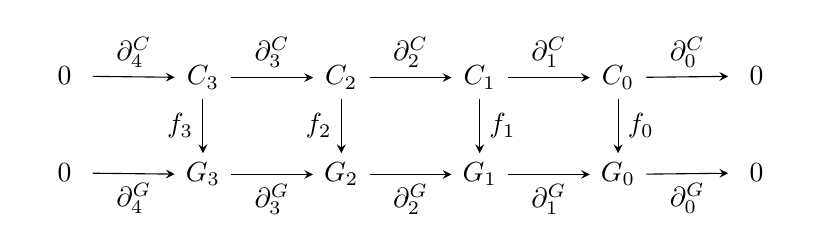
\begin{tikzpicture}
  \matrix (m) [matrix of math nodes,row sep=2em,column sep=3em,minimum width=2em]
  {   0 & C_{3} & C_{2} & C_{1} & C_{0} & 0  \\
      0 & G_3 & G_{2} & G_{1} & G_{0} & 0  \\};
  \path[-stealth]
    (m-1-1) edge node [above] {$\partial^C_{4}$} (m-1-2) 
    (m-1-2) edge node [above] {$\partial^C_{3}$} (m-1-3)
            edge node [left] {$f_3$} (m-2-2)
    (m-1-3) edge node [above] {$\partial^C_{2}$} (m-1-4)
    		edge node [left] {$f_{2}$} (m-2-3)
    (m-1-4) edge node [above] {$\partial^C_{1}$} (m-1-5)
    (m-1-5) edge node [above] {$\partial^C_{0}$} (m-1-6)
    (m-1-5) edge node [right] {$f_0$} (m-2-5)
    (m-1-4) edge node [right] {$f_{1}$} (m-2-4)
    (m-2-1) edge node [below] {$\partial^G_{4}$} (m-2-2)
    (m-2-2) edge node [below] {$\partial^G_{3}$} (m-2-3)
    (m-2-3) edge node [below] {$\partial^G_{2} $} (m-2-4)
    (m-2-4) edge node [below] {$\partial^G_{1}$} (m-2-5)
    (m-2-5) edge node [below] {$\partial^G_{0}$} (m-2-6);
\end{tikzpicture}
\caption{\label{fig:0Gconf} A classical gauge configuration of the gauge theory that includes 0-gauge degrees of freedom.}
\end{figure}

Notice that in Fig.(\ref{fig:0Gconf}) we also considered 1,2 and 3-gauge fields, which is the most general case in 3 spatial dimensions, and we call it \emph{full gauge theory}. Nevertheless, we can arbitrarily set the \(f_i\) maps to be trivial for any \(i= 0,1,2,3\), in the case when the diagram has only one non trivial component \(f_j\), we call the theory a \emph{pure} \(j\)\emph{-gauge} theory.   


The most general case of having an $n$-dimensional complex and placing gauge fields at each dimensional cell is described in detail in \cite{higher,quali}, where we also show that the most efficient way of treating these models is by using the language of homological algebra; This, as well, allows us to completely characterize the ground state subspace in terms of a topological invariant, which is the main result of \cite{higher}. We do not include this formalism here as it is already described in detail in \cite{quali}. 
\end{rem}

\subsection{Geometrical States of Arbitrary Dimensional Many-body Hamiltonians}\label{sec:2.1}

Roughly speaking, the model consists in a 1-gauge theory whose Hilbert space gets now decorated by classical 2-gauge configurations, as we will see. So, we consider a 1-gauge theory defined over an arbitrary (finite) dimensional lattice that can come from a simplicial complex, for instance. The Hilbert space is $\mathcal{H}_\xi :=\bigotimes_{l \in K_1} \mathbb{C}[G_1]_l$, where $\xi: C_2 \rightarrow  G_2$ is a classical configuration (coloring) of degrees of freedom at plaquettes $p \in K_2$ taking values in the Abelian group $G_2$. Moreover, we consider the group homomorphism, $\partial: G_2 \rightarrow G_1$.
The Hamiltonian of the model is given by:
\begin{equation}\label{eq:Hgeo}
H(\xi) = - \sum_{p\in K_2} B_p(\xi) - \sum_{v \in K_0} A_v,
\end{equation}
where the $A_v$ is the usual gauge transformation of a 1-gauge theory, eq. (\ref{eq:Av1G}).On the other hand, the holonomy measurement operator gets modified because of the classical configurations living at plaquettes of the complex. The operator will be, instead, similar to its 2-gauge counterpart, of eq. (\ref{eq:Bp2G}), i.e.,
\begin{align}\label{eq:Bp2G}
 B_p(\xi) \quad \vcenter{\hbox{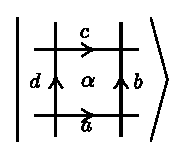
\includegraphics[scale=0.65]{Bp2Gket1.eps}}}\ &= \delta(abc^{-1}d^{-1},\partial(\alpha))\ \vcenter{\hbox{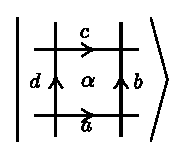
\includegraphics[scale=0.65]{Bp2Gket1.eps}}},
\end{align}
notice that in this case the 2-gauge parameter, $\alpha \in G_2$ is now fixed by the classical configuration $\xi(p)=\alpha$, and it is not dynamical as in the full 2-gauge theory (cf. \S \ref{sec:2gauge}). 

The model can be thought of as being a 2-gauge theory whose plaquette degrees of freedom are now fixed. The fixing of the 2-gauge fields is carried out via the $\xi$ maps. Thus, we are actually dealing with a family of Hamiltonians parametrized by the $\xi$ maps. The role that was being played by the 2-gauge transformation, eq. (\ref{eq:Av2G}), is now split into two transformations that divide the family Hamiltonians into equivalence classes. 

\begin{defn}\label{def:coltrans}
Given a 1-cell (link) $l \in K_1$ and an element $\beta \in G_2$, we define the \emph{color transformation} $T_l(\beta):\xi \rightarrow \xi^{\prime}$, where $\xi$ and $\xi^{\prime}$ are two 2-gauge classical configurations that differ by $T_l(\beta)$ as follows:

\begin{figure}[h!]
\centering
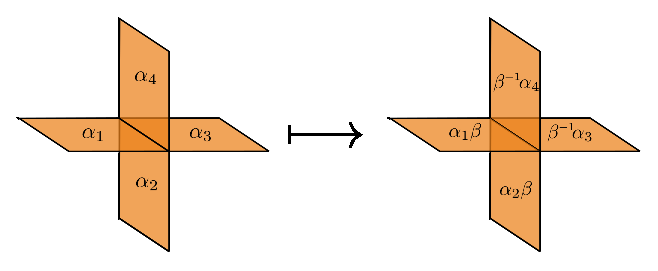
\includegraphics[scale=0.8]{color2G.eps}
\label{fig:coltrans}
\end{figure}

This is, the colorings of the faces around the link $l \in K_1$ are all transformed by the parameter $\beta$ according to the orientations. 
\end{defn}
It is important to emphasize that the above transformation is NOT a 2-gauge transformation, as it is actually mapping between different Hamiltonians. So, in general, for two different colorings $\xi$ and $\xi^{\prime}$ their corresponding Hamiltonians are different, i.e., $H(\xi)\neq H(\xi^{\prime})$. However, if the two colorings, $\xi$ and $\xi^{\prime}$, differ from one another by a color transformation $T_l(\beta)$ (or a sequence of them), it can be shown that the two corresponding Hamiltonians are unitarily equivalent. To achieve this goal, we define the following unitary transformation.
\begin{defn}\label{def:unitrans} Let $l \in K_1$ be an arbitrary 1-cell, a parameter $\beta \in G_2$ and a basis element $\ket{g}\in \mathcal{H}_l$, $g \in G_1$; The \emph{unitary} transformation $U_l(\beta):\mathcal{H}_\xi \rightarrow \mathcal{H}_{\xi^{\prime}}$ is given by:
\[U_l(\beta)\ket{g}=\ket{\partial(\beta)g},\]
where $\partial:G_2 \rightarrow G_1$.
\end{defn}

It is worthwhile pointing out that, in the above definition, both $\mathcal{H}_\xi$ and $\mathcal{H}_{\xi^{\prime}}$ are actually the same Hilbert space, we just write the subscript to highlight the fact that the transformation corresponds to a mutation of colorings from $\xi$ to $\xi^{\prime}$. 
\begin{prop} Let $\xi$ and $\xi^{\prime}$ are two colorings, connected by $T_l(\beta)$ for a given $l \in K_1$. Then, the two Hamiltonians $H(\xi)$ and $H(\xi^{\prime})$ are unitarily equivalent, this is,
\[U_l^{-1}(\beta)H(\xi^{\prime})U_l(\beta) = H(\xi).\]
\end{prop}
\begin{proof}
To show that the above proposition is true, we only need to prove the following:
\[U_l^{-1}(\beta)B_p(\xi^{\prime})U_l(\beta) = B_p(\xi),\]
for all plaquettes $p \in K_2$ adjacent to the link $l$, or more precisely, that have the link $l$ as a boundary. Which follows straightforwardly from applying the definition \ref{def:unitrans} and the definition of the plaquette operator of eq. (\ref{eq:Bp2G}).
\end{proof}
From this unitary equivalence we are able to identify the different equivalence classes of models.
We now turn into an specific example in order to see the geometrical properties of the models. 

\begin{exmp}
We define the model over a lattice that can come from a simplicial complex of a 3 dimensional manifold $\mathcal{M}$, homeomorphic to $S_2 \times I$, such that it has a shortest (dual) path $\gamma$ between the two boundaries:
\begin{figure}[h!]
\centering
    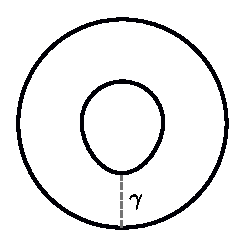
\includegraphics[scale=0.7]{shortest.eps}

\end{figure}

The requirement of having this shortest path is arbitrary and we make this assumption in order to precisely exhibit the main feature of the model. Furthermore, we consider the groups as being $G_1=G_2=\mathbb{Z}_2=\{1,-1\}$ together with the group homomorphism $\partial:\mathbb{Z}_2 \xrightarrow{id} \mathbb{Z}_2$. So we're dealing with a $\mathbb{Z}_2$ 1-gauge theory with classical fields at faces taking values in $\mathbb{Z}_2$, as well. Consequently, the Hilbert space of the model is $\mathcal{H}:=\bigotimes_{l}\mathbb{C}[\mathbb{Z}_2]_l$; An arbitrary basis state $\ket{\psi} \in \mathcal{H}$ consists of spins configurations that will be represented by red (dual) surfaces or the lack of them. We choose this representation as it is best suited for our purpose of exhibiting the ground state in terms of surfaces and strings. For instance, the following configuration:
\begin{figure}[h!]
\centering
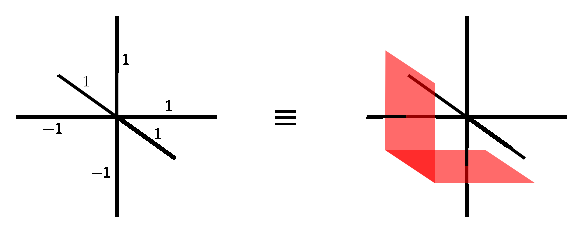
\includegraphics[scale=0.8]{graphstate.eps}
\end{figure}

where the $\ket{-1}$ configurations are represented by dual red surfaces. On the same spirit, we will also use a graphical notation for the coloring of the Hamiltonian  represented in the lattice as green (dual) strings, this is, strings going through faces of the lattice; We would like to emphasize that in this case, we are thinking of the maps $\xi:C_2 \rightarrow G_2$ as decorating the lattice with (dual) strings; These strings are NOT representations of states as the local Hilbert spaces live on the links of the lattice only, for instance, the two possible color configurations on a plaquette are shown in Fig.\ref{fig:plaqconfig}.

\begin{figure}[h!]
\centering
\subfigure[]{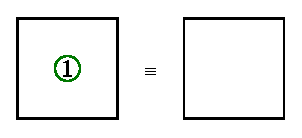
\includegraphics[scale=0.65]{col1.eps}}\hspace{30pt}
\subfigure[]{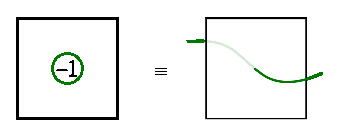
\includegraphics[scale=0.65]{col2.eps}}
\caption{\label{fig:plaqconfig} The two possible colorings at a single plaquette are shown.}
\end{figure}

The vertex operator, $A_v$, that implements local gauge transformations is composed of two parts: 
\[A_v=\dfrac{1}{2}(A_v^{1}+A_v^{-1}),\]
where $A_v^1=\mathbb{1}$ and the action of $A_v^{-1}$ is to flip the configurations from $\ket{1}$ to $\ket{-1}$ and vice versa, around the vertex in question. Concerning our representation of surfaces, the action of local gauge transformations is to either create red spheres or to modify surfaces by isotopy. 

The plaquette operator, $B_p(\xi)$, projects into the "flat"-holonomy subspace of $\mathcal{H}$. Notice that, since they depend on the coloring $\xi$, the configurations that are considered "flat" depend now on the coloring of the lattice. When the coloring is trivial, this is, $\xi(p)=1,\ \forall p \in K_2$, the plaquette operator favors configurations with and even number (or zero) of surfaces around a plaquette. A consequence of this is that, overall, the "flat" sector corresponds to configurations of closed surfaces in the bulk that can open in the each of the boundaries of $\mathcal{M}$. We will refer to this case ($\xi(p)=1,\ \forall p \in K_2$) as \emph{trivial} as it corresponds to defining the Toric Code \cite{Kitaev1} on $\mathcal{M}$. There are, however, colorings that are different from the trivial one, where some or many plaquettes might have a $-1$ coloring attached to it. In the case a particular plaquette $p \in K_2$ has such a coloring, the corresponding plaquette operator will project states different from the trivial case. For instance, the following state:
\begin{align*}
 B_p \quad \vcenter{\hbox{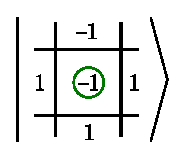
\includegraphics[scale=0.65]{Bket1.eps}}}\ = \delta(1(-1)11,-1)&\  \vcenter{\hbox{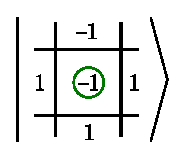
\includegraphics[scale=0.65]{Bket1.eps}}},\\
 = &\vcenter{\hbox{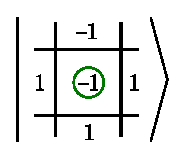
\includegraphics[scale=0.65]{Bket1.eps}}},
\end{align*}
the state has a single link configuration with $\ket{-1}$ yet the plaquette operator is giving a eigenvalue of 1. This particular configuration would not be considered as "flat" in the trivial theory. In our graphical notation, this state would look like:
\begin{figure}[h!]
\centering
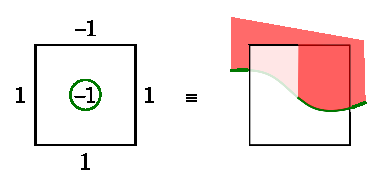
\includegraphics[scale=0.8]{graph2.eps}
\end{figure}
\end{exmp}
The above shows that open surfaces in the bulk are allowed, as long as they end on a green (dual) string, this modifies the dynamics of the model with respect to the trivial case and in particular, the nature of the ground states. To understand this let us look at the different unitary classes of Hamiltonians there are. Hamiltonian of eq.(\ref{eq:Hgeo}) depends on the way the lattice is decorated, given by the maps $\xi$. In principle, different colorings of the lattice give rise to different models; This is true, up to equivalence classes. 
The reason is the existence of both the color transformation of Def. \ref{def:coltrans} and the unitary transformation of Def.\ref{def:unitrans}, to see this let us study the action of both transformations on the colorings and the states. By looking at Def.\ref{def:coltrans} we note that the color transformations are labeled by \(G_2= \mathbb{Z}_2\); Therefore, for a given link \(l \in K_1\) there are two elementary color transformations, namely, \(T_l(1)= \text{id}\) and \(T_l(-1)\) that flips the configurations at plaquettes around \(l\), as shown in Def. \ref{def:coltrans}. Thus, the only non trivial action of the color transformation is given by \(T_l(-1)\) and can thought of as either creating a closed (dual) string around the link \(l\) or extending an existing string by local isotopy, as shown in Fig.(\ref{fig:coltrans}).
With this information we are able to explore the equivalence classes of Hamiltonians. The color transformation can only add closed dual strings or extend existing ones by isotopy; Also, considering that closed dual strings on the bulk can be opened at the two boundaries of \(\mathcal{M}\) it is nor difficult to realize that there are two unitary equivalence classes of Hamiltonians.

\begin{figure}[h!]
\centering
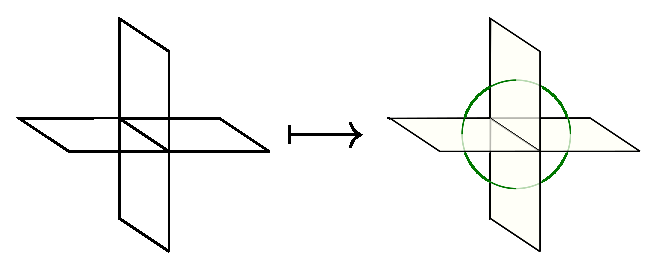
\includegraphics[scale=0.6]{coltrans.eps}
\caption{\label{fig:coltrans}Color transformation around a link.}
\end{figure}

\textbf{Class 1.-} This class corresponds to the trivial coloring model, i.e., all colorings that are unitarily equivalent to the model with trivial coloring. The equivalence class corresponds to having an even number of dual strings connecting the two boundaries, as it is shown in Fig. \ref{fig:class1}. This class of models correspond to defining the Toric Code on the manifold \(\mathcal{M}\). We wont dwell onto the details of this class of models since they are all known as they correspond to the usual topological models. A detailed description will be found on \cite{pablo}.
\begin{figure}[h!]
\centering
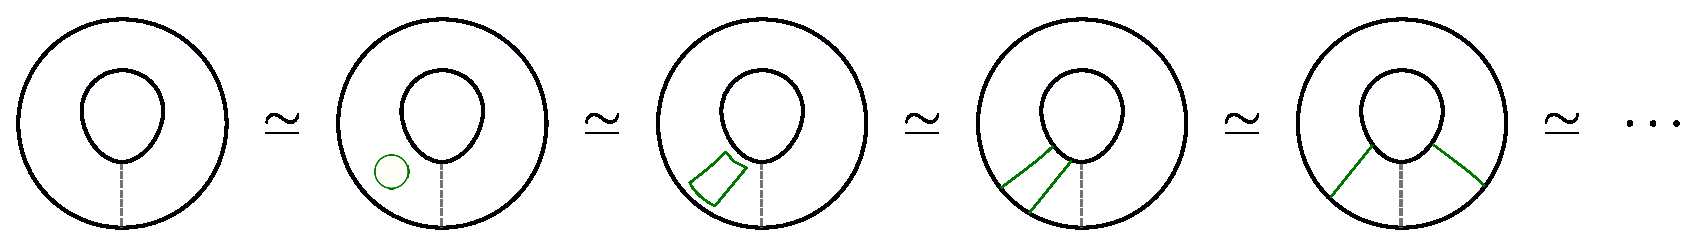
\includegraphics[scale=0.55]{class1.eps}
\caption{\label{fig:class1}Some equivalent colorings of class 1 are shown.}
\end{figure}

\textbf{Class 2.-} This class consists on all lattice colorings that have an odd number of strings connecting the two boundaries of \(\mathcal{M}\), as shown in Fig.\ref{fig:class2}. This is the class of models that we are interested in, consequently we will give a preliminary analysis of the ground state subspace of such models. First of all, we know is sufficient to take a representative of the class and we will work with the coloring with one single dual string connecting the two surfaces.
\begin{figure}[h!]
\centering
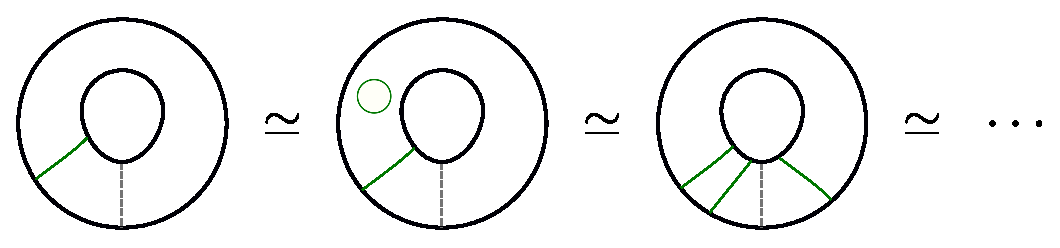
\includegraphics[scale=0.55]{class2.eps}
\caption{\label{fig:class2}Some equivalent colorings of class 2 are shown.}
\end{figure}

To study the ground state of the model we first notice that all plaquettes being crossed by the string will project to the holonomy value of \(-1\). Therefore, if we take the coloring of the representative in Fig.\ref{fig:class2} and consider the seed state with \(\ket{1}\) at every link, the following state:
\[\ket{\psi}= \prod_v A_v\ \ \vcenter{\hbox{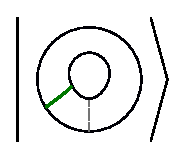
\includegraphics[scale=0.65]{ket1.eps}}}\ ,\]
has an energy proportional to the length\footnote{By length we mean the number of plaquettes being crossed by the string.}, \(l_p\), of the string. This can be seen from the eigenvalues of the plaquette operators affected by the coloring:
\[B_p\ \ \vcenter{\hbox{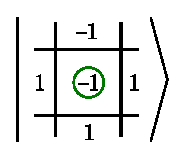
\includegraphics[scale=0.65]{Bket1.eps}}} = \delta(1111,-1)\ \ \vcenter{\hbox{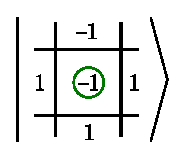
\includegraphics[scale=0.65]{Bket1.eps}}}=0\ ,\]
therefore evaluating the Hamiltonian operator on this state we obtain:
\begin{equation}\label{eq:Epsi}
H\ket{\psi}=-(N_v -(N_p - l_p))\ket{\psi},
\end{equation}

where \(N_v= |K_0|\) and \(N_p=|K_2|\) are the number of vertices and plaquettes, respectively.
hence, it is clear that the energy of such a state depends linearly on the length of the string. Naturally, arises the question of whether it exists a state with less energy than \(\ket{\psi}\). We recall that the minimum energy in the topological case (class 1) is \(E_0=-N_v - N_p\), thus we can also ask if whether this is the energy minimum for the Hamiltonians of class 2. The answer to both questions is obtained by looking at the details of \(\mathcal{M}\), recall that the lattice we over which the model is defined has a shortest dual path \(\gamma\) that joins the two surfaces. Thus, if we consider the following state,
\[\ket{\psi_0}= \prod_v A_v \ \ \vcenter{\hbox{
\includegraphics[scale=0.65]{ket2.eps}}}\ ,\]
that consists on a red surface extending from the coloring string to the shortest path. Evaluating the Hamiltonian operator over this state we obtain,
\begin{equation}\label{eq:Epsi0}
H\ket{\psi_0}=-(N_v -(N_p - \gamma_p))\ket{\psi_0}, 
\end{equation}
now, we  know that \(\gamma_p  < l_p\) for any dual string length \(l_p\). Therefore,  \(\ket{\psi_0}\) is the state with least energy in \(\mathcal{H}\).
We want to stress that no matter what representative of the class of Hamiltonians we choose, the ground state will still perform the same task, this is, to find the shortest path between the two surfaces. Notice that, to localize this path it is enough to act with plaquette operators and look for the ones that get excited. As one can see in eqns. (\ref{eq:Epsi}) and (\ref{eq:Epsi0}), the energy of these states is bigger than the ground state energy of the Hamiltonians in class 1, this is due to the existence of a single dual string on the lattice. To understand this let us look at the concrete action of the coloring $\xi$ on the dynamics of the models; The dual string modifies the plaquette operators on its path making them project to the $-1$ sector, this can be thought of as condensing flux excitations at these plaquettes. However, flux excitations in the (trivial) theory always come in pairs, concretely pairs of dual strings (up to gauge transformations). Then by condensing one of the strings at the modified plaquettes there is one single dual string of excitations left "free". The ground state of the models consist on placing this "free" dual string at the shortest (dual) path from one inner to the outer surfaces, thus minimizing the energy of the state. 

We see that even on the simplest example we get rich new behavior both for the ground states and the excited states. The geometric property of the ground state makes us place these models into what is known as fracton phases \cite{chamon05,rahul18}. Moreover, the procedure of making classical some degrees of freedom  of a higher gauge theory we have a plethora of models with similar phenomena. The construction can be carried out for arbitrary dimensions and gauge fields. The goal of the Ph.D. thesis manuscript is to condense all these models and phenomena in a rigorous and concrete way. To do so, we sketch the future work schedule that will be followed until the finishing of the manuscript.


\section{Future Work Schedule}
In the following academic period our main objective is to finish the Ph. D. thesis while sticking to the following activity schedule, 
\begin{enumerate}
\item To continue with the systematic bibliographic revision concerning the following topics: Topological phases of matter in arbitrary dimensions, Topological Quantum Field Theories and their relation with lattice models for topological phases in arbitrary dimensions, fracton phases of matter, entanglement entropy of fracton phases among others.
\item To prove that there is no state with energy less than $\ket{\psi_0}.$
\item To study the low energy excited states and their mobility properties .
\item To extend the construction for higher and lower dimensional gauge fields.
\item To fit the construction in the homological algebra formalism of \cite{higher}
\item To finish \cite{higher} and \cite{pablo}.
\item To finish the thesis.

\end{enumerate}

\section{Academic Activities}
\begin{itemize}
\item During the II-2017 academic term:
The student did not attend any course. 

In 09/11/2017, the student was approved in the Ph. D. Qualifying Exam (manuscript annexed).

Also, the student attended the following school held at the \emph{International Centre for Theoretical Physics - South American Institute Fundamental Research } (ICTP-SAIFR): \textbf{Minicourse on Machine Learning for Many-Body Physics}.
\item During the I-2018 academic term, the student attended the following school held at the \emph{Universidad de los Andes - Bogotá}: \textbf{School on Mathematical Physics: Topological Order and Beyond}.

\end{itemize}

\bibliographystyle{unsrt}
%\bibliographystyle{model1-num-names}
\bibliography{sample.bib}

\end{document}